\documentclass[twoside]{book}

% Packages required by doxygen
\usepackage{fixltx2e}
\usepackage{calc}
\usepackage{doxygen}
\usepackage[export]{adjustbox} % also loads graphicx
\usepackage{graphicx}
\usepackage[utf8]{inputenc}
\usepackage{makeidx}
\usepackage{multicol}
\usepackage{multirow}
\PassOptionsToPackage{warn}{textcomp}
\usepackage{textcomp}
\usepackage[nointegrals]{wasysym}
\usepackage[table]{xcolor}

% NLS support packages
\usepackage[spanish]{babel}
% Font selection
\usepackage[T1]{fontenc}
\usepackage[scaled=.90]{helvet}
\usepackage{courier}
\usepackage{amssymb}
\usepackage{sectsty}
\renewcommand{\familydefault}{\sfdefault}
\allsectionsfont{%
  \fontseries{bc}\selectfont%
  \color{darkgray}%
}
\renewcommand{\DoxyLabelFont}{%
  \fontseries{bc}\selectfont%
  \color{darkgray}%
}
\newcommand{\+}{\discretionary{\mbox{\scriptsize$\hookleftarrow$}}{}{}}

% Page & text layout
\usepackage{geometry}
\geometry{%
  a4paper,%
  top=2.5cm,%
  bottom=2.5cm,%
  left=2.5cm,%
  right=2.5cm%
}
\tolerance=750
\hfuzz=15pt
\hbadness=750
\setlength{\emergencystretch}{15pt}
\setlength{\parindent}{0cm}
\setlength{\parskip}{3ex plus 2ex minus 2ex}
\makeatletter
\renewcommand{\paragraph}{%
  \@startsection{paragraph}{4}{0ex}{-1.0ex}{1.0ex}{%
    \normalfont\normalsize\bfseries\SS@parafont%
  }%
}
\renewcommand{\subparagraph}{%
  \@startsection{subparagraph}{5}{0ex}{-1.0ex}{1.0ex}{%
    \normalfont\normalsize\bfseries\SS@subparafont%
  }%
}
\makeatother

% Headers & footers
\usepackage{fancyhdr}
\pagestyle{fancyplain}
\fancyhead[LE]{\fancyplain{}{\bfseries\thepage}}
\fancyhead[CE]{\fancyplain{}{}}
\fancyhead[RE]{\fancyplain{}{\bfseries\leftmark}}
\fancyhead[LO]{\fancyplain{}{\bfseries\rightmark}}
\fancyhead[CO]{\fancyplain{}{}}
\fancyhead[RO]{\fancyplain{}{\bfseries\thepage}}
\fancyfoot[LE]{\fancyplain{}{}}
\fancyfoot[CE]{\fancyplain{}{}}
\fancyfoot[RE]{\fancyplain{}{\bfseries\scriptsize Generado por Doxygen }}
\fancyfoot[LO]{\fancyplain{}{\bfseries\scriptsize Generado por Doxygen }}
\fancyfoot[CO]{\fancyplain{}{}}
\fancyfoot[RO]{\fancyplain{}{}}
\renewcommand{\footrulewidth}{0.4pt}
\renewcommand{\chaptermark}[1]{%
  \markboth{#1}{}%
}
\renewcommand{\sectionmark}[1]{%
  \markright{\thesection\ #1}%
}

% Indices & bibliography
\usepackage{natbib}
\usepackage[titles]{tocloft}
\setcounter{tocdepth}{3}
\setcounter{secnumdepth}{5}
\makeindex

% Hyperlinks (required, but should be loaded last)
\usepackage{ifpdf}
\ifpdf
  \usepackage[pdftex,pagebackref=true]{hyperref}
\else
  \usepackage[ps2pdf,pagebackref=true]{hyperref}
\fi
\hypersetup{%
  colorlinks=true,%
  linkcolor=blue,%
  citecolor=blue,%
  unicode%
}

% Custom commands
\newcommand{\clearemptydoublepage}{%
  \newpage{\pagestyle{empty}\cleardoublepage}%
}

\usepackage{caption}
\captionsetup{labelsep=space,justification=centering,font={bf},singlelinecheck=off,skip=4pt,position=top}

%===== C O N T E N T S =====

\begin{document}

% Titlepage & ToC
\hypersetup{pageanchor=false,
             bookmarksnumbered=true,
             pdfencoding=unicode
            }
\pagenumbering{roman}
\begin{titlepage}
\vspace*{7cm}
\begin{center}%
{\Large Circulo medio \\[1ex]\large 0 }\\
\vspace*{1cm}
{\large Generado por Doxygen 1.8.11}\\
\end{center}
\end{titlepage}
\clearemptydoublepage
\tableofcontents
\clearemptydoublepage
\pagenumbering{arabic}
\hypersetup{pageanchor=true}

%--- Begin generated contents ---
\chapter{Índice de clases}
\section{Lista de clases}
Lista de las clases, estructuras, uniones e interfaces con una breve descripción\+:\begin{DoxyCompactList}
\item\contentsline{section}{\hyperlink{classCirculo}{Circulo} \\*Clase Círculo }{\pageref{classCirculo}}{}
\item\contentsline{section}{\hyperlink{classPunto}{Punto} \\*Clase \hyperlink{classPunto}{Punto} }{\pageref{classPunto}}{}
\end{DoxyCompactList}

\chapter{Indice de archivos}
\section{Lista de archivos}
Lista de todos los archivos documentados y con descripciones breves\+:\begin{DoxyCompactList}
\item\contentsline{section}{\hyperlink{circulomedio_8cpp}{circulomedio.\+cpp} \\*Calcula círculo con centro en medio de dos círculos y radio la mitad de la distancia }{\pageref{circulomedio_8cpp}}{}
\end{DoxyCompactList}

\chapter{Documentación de las clases}
\hypertarget{classCirculo}{}\section{Referencia de la Clase Circulo}
\label{classCirculo}\index{Circulo@{Circulo}}


Clase Círculo.  




Diagrama de colaboración para Circulo\+:\nopagebreak
\begin{figure}[H]
\begin{center}
\leavevmode
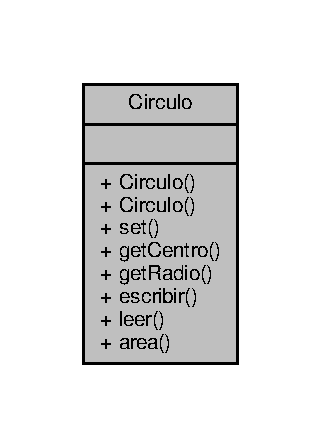
\includegraphics[width=154pt]{classCirculo__coll__graph}
\end{center}
\end{figure}
\subsection*{Métodos públicos}
\begin{DoxyCompactItemize}
\item 
\hyperlink{classCirculo_a6933bf908b78a4167684081a3a8f257f}{Circulo} ()\hypertarget{classCirculo_a6933bf908b78a4167684081a3a8f257f}{}\label{classCirculo_a6933bf908b78a4167684081a3a8f257f}

\begin{DoxyCompactList}\small\item\em Constructor\+: Pone a 0 el punto y el radio. \end{DoxyCompactList}\item 
\hyperlink{classCirculo_ad4c6c76f0227c25afcb872a8744ebe56}{Circulo} (\hyperlink{classPunto}{Punto} centro, double radio)\hypertarget{classCirculo_ad4c6c76f0227c25afcb872a8744ebe56}{}\label{classCirculo_ad4c6c76f0227c25afcb872a8744ebe56}

\begin{DoxyCompactList}\small\item\em Constructor\+: Inicializa el círculo con un centro y un radio. \end{DoxyCompactList}\item 
void \hyperlink{classCirculo_aa24cc4b316a3d9ece35f120d9b8e1fc4}{set} (\hyperlink{classPunto}{Punto} centro, double radio)\hypertarget{classCirculo_aa24cc4b316a3d9ece35f120d9b8e1fc4}{}\label{classCirculo_aa24cc4b316a3d9ece35f120d9b8e1fc4}

\begin{DoxyCompactList}\small\item\em Asigna el centro y el radio a un circulo. \end{DoxyCompactList}\item 
\hyperlink{classPunto}{Punto} \hyperlink{classCirculo_a022cde4d10d14a47a3b3921f80909f3b}{get\+Centro} () const \hypertarget{classCirculo_a022cde4d10d14a47a3b3921f80909f3b}{}\label{classCirculo_a022cde4d10d14a47a3b3921f80909f3b}

\begin{DoxyCompactList}\small\item\em Devuelve el centro de un circulo. \end{DoxyCompactList}\item 
double \hyperlink{classCirculo_a982f8a785d8a68ab1483b609cd752980}{get\+Radio} () const \hypertarget{classCirculo_a982f8a785d8a68ab1483b609cd752980}{}\label{classCirculo_a982f8a785d8a68ab1483b609cd752980}

\begin{DoxyCompactList}\small\item\em Devuelve el radio de un circulo. \end{DoxyCompactList}\item 
void \hyperlink{classCirculo_a2deaed49ea394702beb0554f9480137e}{escribir} () const \hypertarget{classCirculo_a2deaed49ea394702beb0554f9480137e}{}\label{classCirculo_a2deaed49ea394702beb0554f9480137e}

\begin{DoxyCompactList}\small\item\em Escribe círculo en formato radio-\/centro. \end{DoxyCompactList}\item 
void \hyperlink{classCirculo_aa71efffb3b42eeaefd43743a8d34aa74}{leer} ()\hypertarget{classCirculo_aa71efffb3b42eeaefd43743a8d34aa74}{}\label{classCirculo_aa71efffb3b42eeaefd43743a8d34aa74}

\begin{DoxyCompactList}\small\item\em lee círculo en formato radio-\/centro \end{DoxyCompactList}\item 
double \hyperlink{classCirculo_a532d4f2bd03b688403c4370319411dc3}{area} () const \hypertarget{classCirculo_a532d4f2bd03b688403c4370319411dc3}{}\label{classCirculo_a532d4f2bd03b688403c4370319411dc3}

\begin{DoxyCompactList}\small\item\em Devuelve el área de un círculo. \end{DoxyCompactList}\end{DoxyCompactItemize}


\subsection{Descripción detallada}
Clase Círculo. 

Definición en la línea 85 del archivo circulomedio.\+cpp.



La documentación para esta clase fue generada a partir del siguiente fichero\+:\begin{DoxyCompactItemize}
\item 
\hyperlink{circulomedio_8cpp}{circulomedio.\+cpp}\end{DoxyCompactItemize}

\hypertarget{classPunto}{}\section{Referencia de la Clase Punto}
\label{classPunto}\index{Punto@{Punto}}


Clase \hyperlink{classPunto}{Punto}.  




Diagrama de colaboración para Punto\+:\nopagebreak
\begin{figure}[H]
\begin{center}
\leavevmode
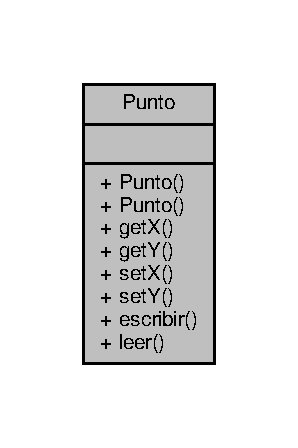
\includegraphics[width=143pt]{classPunto__coll__graph}
\end{center}
\end{figure}
\subsection*{Métodos públicos}
\begin{DoxyCompactItemize}
\item 
\hyperlink{classPunto_a4b8b70b933ff13493ee5ddb3c8532c10}{Punto} ()\hypertarget{classPunto_a4b8b70b933ff13493ee5ddb3c8532c10}{}\label{classPunto_a4b8b70b933ff13493ee5ddb3c8532c10}

\begin{DoxyCompactList}\small\item\em constructor. Pone a 0 las dos coordenadas \end{DoxyCompactList}\item 
\hyperlink{classPunto_a91b4238ec1ca3ddfb7b60b601a908d25}{Punto} (double \+\_\+x, double \+\_\+y)\hypertarget{classPunto_a91b4238ec1ca3ddfb7b60b601a908d25}{}\label{classPunto_a91b4238ec1ca3ddfb7b60b601a908d25}

\begin{DoxyCompactList}\small\item\em constructor. Inicializa un punto con dos valores x y \end{DoxyCompactList}\item 
double \hyperlink{classPunto_aa218292fec9bad5ec6d71d4bd9173d9d}{getX} () const \hypertarget{classPunto_aa218292fec9bad5ec6d71d4bd9173d9d}{}\label{classPunto_aa218292fec9bad5ec6d71d4bd9173d9d}

\begin{DoxyCompactList}\small\item\em Devuelve la coordenada x del punto. \end{DoxyCompactList}\item 
double \hyperlink{classPunto_a214978b8bbae48ca5927f2e56fb3bd22}{getY} () const \hypertarget{classPunto_a214978b8bbae48ca5927f2e56fb3bd22}{}\label{classPunto_a214978b8bbae48ca5927f2e56fb3bd22}

\begin{DoxyCompactList}\small\item\em Devuelve la coordenada y del punto. \end{DoxyCompactList}\item 
void \hyperlink{classPunto_a51ae6616f828bb2b4111bc8ace49dbca}{setX} (double nuevoX)\hypertarget{classPunto_a51ae6616f828bb2b4111bc8ace49dbca}{}\label{classPunto_a51ae6616f828bb2b4111bc8ace49dbca}

\begin{DoxyCompactList}\small\item\em Asigna el valor nuevoX a la coordenada x del punto. \end{DoxyCompactList}\item 
void \hyperlink{classPunto_a6a0f8adb5946f31a7867a06f54d97462}{setY} (double nuevoY)\hypertarget{classPunto_a6a0f8adb5946f31a7867a06f54d97462}{}\label{classPunto_a6a0f8adb5946f31a7867a06f54d97462}

\begin{DoxyCompactList}\small\item\em Asigna el valor nuevoY a la coordenada y del punto. \end{DoxyCompactList}\item 
void \hyperlink{classPunto_afc543b48134f632fa354d8b027954e80}{escribir} () const \hypertarget{classPunto_afc543b48134f632fa354d8b027954e80}{}\label{classPunto_afc543b48134f632fa354d8b027954e80}

\begin{DoxyCompactList}\small\item\em Escribe un punto en formato (x,y) \end{DoxyCompactList}\item 
void \hyperlink{classPunto_a84cc9b0ee2e5b00842e7bff819b80459}{leer} ()\hypertarget{classPunto_a84cc9b0ee2e5b00842e7bff819b80459}{}\label{classPunto_a84cc9b0ee2e5b00842e7bff819b80459}

\begin{DoxyCompactList}\small\item\em // Lee un punto en el formato (x,y) \end{DoxyCompactList}\end{DoxyCompactItemize}


\subsection{Descripción detallada}
Clase \hyperlink{classPunto}{Punto}. 

Definición en la línea 18 del archivo circulomedio.\+cpp.



La documentación para esta clase fue generada a partir del siguiente fichero\+:\begin{DoxyCompactItemize}
\item 
\hyperlink{circulomedio_8cpp}{circulomedio.\+cpp}\end{DoxyCompactItemize}

\chapter{Documentación de archivos}
\hypertarget{circulomedio_8cpp}{}\section{Referencia del Archivo circulomedio.\+cpp}
\label{circulomedio_8cpp}\index{circulomedio.\+cpp@{circulomedio.\+cpp}}


Calcula círculo con centro en medio de dos círculos y radio la mitad de la distancia.  


{\ttfamily \#include $<$iostream$>$}\\*
{\ttfamily \#include $<$cmath$>$}\\*
Dependencia gráfica adjunta para circulomedio.\+cpp\+:
\nopagebreak
\begin{figure}[H]
\begin{center}
\leavevmode
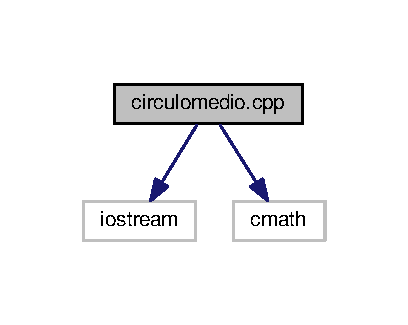
\includegraphics[width=196pt]{circulomedio_8cpp__incl}
\end{center}
\end{figure}
\subsection*{Clases}
\begin{DoxyCompactItemize}
\item 
class \hyperlink{classPunto}{Punto}
\begin{DoxyCompactList}\small\item\em Clase \hyperlink{classPunto}{Punto}. \end{DoxyCompactList}\item 
class \hyperlink{classCirculo}{Circulo}
\begin{DoxyCompactList}\small\item\em Clase Círculo. \end{DoxyCompactList}\end{DoxyCompactItemize}
\subsection*{Funciones}
\begin{DoxyCompactItemize}
\item 
double \hyperlink{circulomedio_8cpp_a9c93fd6721d3b594dbbcfb77a92a2880}{distancia} (\hyperlink{classPunto}{Punto} p1, \hyperlink{classPunto}{Punto} p2)
\begin{DoxyCompactList}\small\item\em Clase \hyperlink{classPunto}{Punto}. \end{DoxyCompactList}\item 
\hyperlink{classPunto}{Punto} \hyperlink{circulomedio_8cpp_a119f914f219e98be4c2c93b5138e97da}{punto\+Medio} (\hyperlink{classPunto}{Punto} p1, \hyperlink{classPunto}{Punto} p2)
\begin{DoxyCompactList}\small\item\em Calcula el punto que está entre dos puntos dados con distancia mínima a ambos. \end{DoxyCompactList}\item 
double \hyperlink{circulomedio_8cpp_a2be093c30676e02d6f76b6a56c713b34}{distancia} (\hyperlink{classCirculo}{Circulo} c1, \hyperlink{classCirculo}{Circulo} c2)
\begin{DoxyCompactList}\small\item\em Clase \hyperlink{classCirculo}{Circulo}. \end{DoxyCompactList}\item 
bool \hyperlink{circulomedio_8cpp_a6e60e1271c0a8f48e87f8e53b434dfd4}{interior} (\hyperlink{classPunto}{Punto} p, \hyperlink{classCirculo}{Circulo} c)
\begin{DoxyCompactList}\small\item\em Comprueba si un punto es interior a un círculo. \end{DoxyCompactList}\item 
int {\bfseries main} ()\hypertarget{circulomedio_8cpp_ae66f6b31b5ad750f1fe042a706a4e3d4}{}\label{circulomedio_8cpp_ae66f6b31b5ad750f1fe042a706a4e3d4}

\end{DoxyCompactItemize}


\subsection{Descripción detallada}
Calcula círculo con centro en medio de dos círculos y radio la mitad de la distancia. 

\begin{DoxyAuthor}{Autor}
MP Grupo B, C 
\end{DoxyAuthor}
\begin{DoxyWarning}{Atención}
Módulo no definitivo (creado para ser modificado)
\end{DoxyWarning}
Un ejemplo de ejecución es\+: Introduzca un circulo en formato radio-\/(x,y)\+: 3-\/(0,0) Introduzca otro circulo\+: 4-\/(5,0) El círculo que pasa por los dos centros es\+: 2.\+5-\/(2.\+5,0) 

\subsection{Documentación de las funciones}
\index{circulomedio.\+cpp@{circulomedio.\+cpp}!distancia@{distancia}}
\index{distancia@{distancia}!circulomedio.\+cpp@{circulomedio.\+cpp}}
\subsubsection[{\texorpdfstring{distancia(\+Punto p1, Punto p2)}{distancia(Punto p1, Punto p2)}}]{\setlength{\rightskip}{0pt plus 5cm}double distancia (
\begin{DoxyParamCaption}
\item[{{\bf Punto}}]{p1, }
\item[{{\bf Punto}}]{p2}
\end{DoxyParamCaption}
)}\hypertarget{circulomedio_8cpp_a9c93fd6721d3b594dbbcfb77a92a2880}{}\label{circulomedio_8cpp_a9c93fd6721d3b594dbbcfb77a92a2880}


Clase \hyperlink{classPunto}{Punto}. 

Funciones auxiliares (no son métodos de la clase) Calcula la distancia entre dos puntos 
\begin{DoxyParams}{Parámetros}
{\em p1} & primer punto \\
\hline
{\em p2} & segundo punto \\
\hline
\end{DoxyParams}
\begin{DoxyReturn}{Devuelve}
la distancia entre el punto {\itshape p1} y el punto {\itshape p2} 
\end{DoxyReturn}


Definición en la línea 63 del archivo circulomedio.\+cpp.


\begin{DoxyCode}
63                                     \{
64     \textcolor{keywordflow}{return} sqrt((p1.\hyperlink{classPunto_aa218292fec9bad5ec6d71d4bd9173d9d}{getX}()-p2.\hyperlink{classPunto_aa218292fec9bad5ec6d71d4bd9173d9d}{getX}())*(p1.\hyperlink{classPunto_aa218292fec9bad5ec6d71d4bd9173d9d}{getX}()-p2.\hyperlink{classPunto_aa218292fec9bad5ec6d71d4bd9173d9d}{getX}()) +
65          (p1.\hyperlink{classPunto_a214978b8bbae48ca5927f2e56fb3bd22}{getY}()-p2.\hyperlink{classPunto_a214978b8bbae48ca5927f2e56fb3bd22}{getY}())*(p1.\hyperlink{classPunto_a214978b8bbae48ca5927f2e56fb3bd22}{getY}()-p2.\hyperlink{classPunto_a214978b8bbae48ca5927f2e56fb3bd22}{getY}()));
66 \}
\end{DoxyCode}


Gráfico de llamadas para esta función\+:
\nopagebreak
\begin{figure}[H]
\begin{center}
\leavevmode
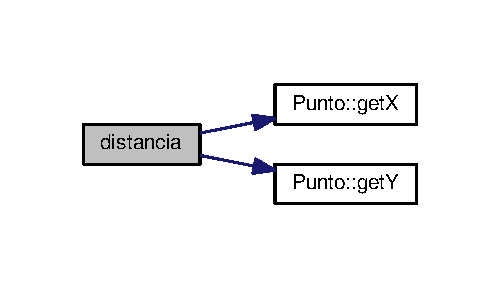
\includegraphics[width=240pt]{circulomedio_8cpp_a9c93fd6721d3b594dbbcfb77a92a2880_cgraph}
\end{center}
\end{figure}


\index{circulomedio.\+cpp@{circulomedio.\+cpp}!distancia@{distancia}}
\index{distancia@{distancia}!circulomedio.\+cpp@{circulomedio.\+cpp}}
\subsubsection[{\texorpdfstring{distancia(\+Circulo c1, Circulo c2)}{distancia(Circulo c1, Circulo c2)}}]{\setlength{\rightskip}{0pt plus 5cm}double distancia (
\begin{DoxyParamCaption}
\item[{{\bf Circulo}}]{c1, }
\item[{{\bf Circulo}}]{c2}
\end{DoxyParamCaption}
)}\hypertarget{circulomedio_8cpp_a2be093c30676e02d6f76b6a56c713b34}{}\label{circulomedio_8cpp_a2be093c30676e02d6f76b6a56c713b34}


Clase \hyperlink{classCirculo}{Circulo}. 

Funciones auxiliares Calcula la distancia entre dos circulos 
\begin{DoxyParams}{Parámetros}
{\em c1} & primer círculo \\
\hline
{\em c2} & segundo círculo \\
\hline
\end{DoxyParams}
\begin{DoxyReturn}{Devuelve}
la distancia entre el círculo {\itshape c1} y el círculo {\itshape c2} 
\end{DoxyReturn}
La distancia entre dos círculos se define como la distancia entre los centros menos los dos radios. Nótese que la distancia puede ser negativa si los círculos se intersecan 

Definición en la línea 156 del archivo circulomedio.\+cpp.


\begin{DoxyCode}
156                                          \{
157     \hyperlink{classPunto}{Punto} centro1, centro2;
158     \textcolor{keywordtype}{double} dist;
159 
160     centro1=c1.\hyperlink{classCirculo_a022cde4d10d14a47a3b3921f80909f3b}{getCentro}();
161     centro2=c2.\hyperlink{classCirculo_a022cde4d10d14a47a3b3921f80909f3b}{getCentro}();
162     dist=\hyperlink{circulomedio_8cpp_a9c93fd6721d3b594dbbcfb77a92a2880}{distancia}(centro1,centro2)-c1.\hyperlink{classCirculo_a982f8a785d8a68ab1483b609cd752980}{getRadio}()-c2.\hyperlink{classCirculo_a982f8a785d8a68ab1483b609cd752980}{getRadio}();
163     \textcolor{keywordflow}{return} dist;
164 \}
\end{DoxyCode}


Gráfico de llamadas para esta función\+:
\nopagebreak
\begin{figure}[H]
\begin{center}
\leavevmode
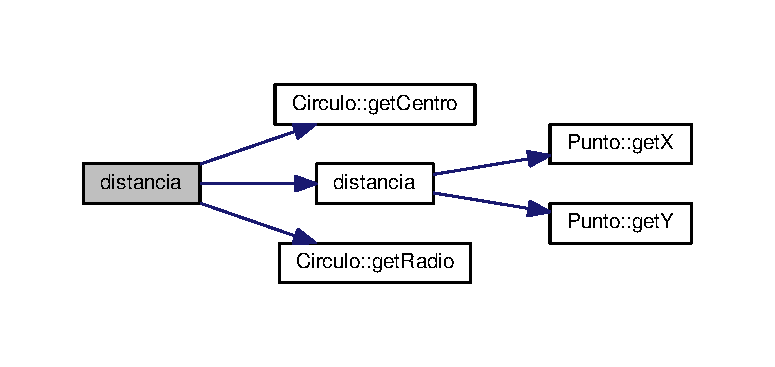
\includegraphics[width=350pt]{circulomedio_8cpp_a2be093c30676e02d6f76b6a56c713b34_cgraph}
\end{center}
\end{figure}


\index{circulomedio.\+cpp@{circulomedio.\+cpp}!interior@{interior}}
\index{interior@{interior}!circulomedio.\+cpp@{circulomedio.\+cpp}}
\subsubsection[{\texorpdfstring{interior(\+Punto p, Circulo c)}{interior(Punto p, Circulo c)}}]{\setlength{\rightskip}{0pt plus 5cm}bool interior (
\begin{DoxyParamCaption}
\item[{{\bf Punto}}]{p, }
\item[{{\bf Circulo}}]{c}
\end{DoxyParamCaption}
)}\hypertarget{circulomedio_8cpp_a6e60e1271c0a8f48e87f8e53b434dfd4}{}\label{circulomedio_8cpp_a6e60e1271c0a8f48e87f8e53b434dfd4}


Comprueba si un punto es interior a un círculo. 


\begin{DoxyParams}{Parámetros}
{\em p} & punto a comprobar \\
\hline
{\em c} & circulo \\
\hline
\end{DoxyParams}

\begin{DoxyRetVals}{Valores devueltos}
{\em true} & si el punto {\itshape p} es interior al círculo {\itshape c} \\
\hline
{\em false} & en caso contrario \\
\hline
\end{DoxyRetVals}


Definición en la línea 174 del archivo circulomedio.\+cpp.


\begin{DoxyCode}
174                                   \{
175     \textcolor{keywordflow}{if}(\hyperlink{circulomedio_8cpp_a9c93fd6721d3b594dbbcfb77a92a2880}{distancia}(p,c.\hyperlink{classCirculo_a022cde4d10d14a47a3b3921f80909f3b}{getCentro}())<=c.\hyperlink{classCirculo_a982f8a785d8a68ab1483b609cd752980}{getRadio}()) \{
176         \textcolor{keywordflow}{return} \textcolor{keyword}{true};
177     \}
178     \textcolor{keywordflow}{else}\{
179         \textcolor{keywordflow}{return} \textcolor{keyword}{false};
180     \}
181 \}
\end{DoxyCode}


Gráfico de llamadas para esta función\+:
\nopagebreak
\begin{figure}[H]
\begin{center}
\leavevmode
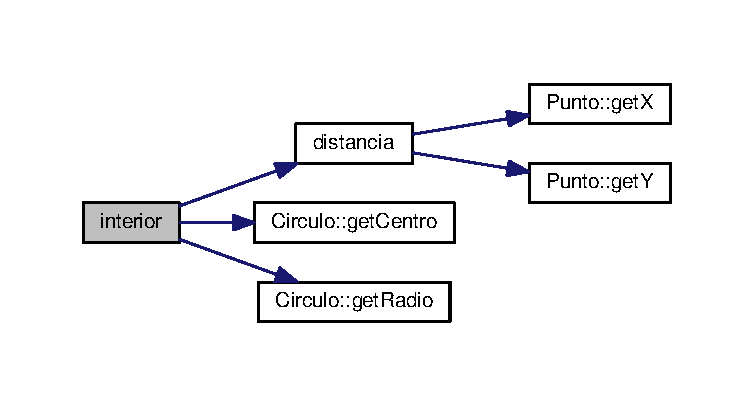
\includegraphics[width=350pt]{circulomedio_8cpp_a6e60e1271c0a8f48e87f8e53b434dfd4_cgraph}
\end{center}
\end{figure}


\index{circulomedio.\+cpp@{circulomedio.\+cpp}!punto\+Medio@{punto\+Medio}}
\index{punto\+Medio@{punto\+Medio}!circulomedio.\+cpp@{circulomedio.\+cpp}}
\subsubsection[{\texorpdfstring{punto\+Medio(\+Punto p1, Punto p2)}{puntoMedio(Punto p1, Punto p2)}}]{\setlength{\rightskip}{0pt plus 5cm}{\bf Punto} punto\+Medio (
\begin{DoxyParamCaption}
\item[{{\bf Punto}}]{p1, }
\item[{{\bf Punto}}]{p2}
\end{DoxyParamCaption}
)}\hypertarget{circulomedio_8cpp_a119f914f219e98be4c2c93b5138e97da}{}\label{circulomedio_8cpp_a119f914f219e98be4c2c93b5138e97da}


Calcula el punto que está entre dos puntos dados con distancia mínima a ambos. 


\begin{DoxyParams}{Parámetros}
{\em p1} & primer punto \\
\hline
{\em p2} & segundo punto \\
\hline
\end{DoxyParams}
\begin{DoxyReturn}{Devuelve}
un punto entre el punto {\itshape p1} y el punto {\itshape p2} con distancia mínima a ambos 
\end{DoxyReturn}


Definición en la línea 76 del archivo circulomedio.\+cpp.


\begin{DoxyCode}
76                                     \{
77     \hyperlink{classPunto}{Punto} pMedio;
78     pMedio.\hyperlink{classPunto_a51ae6616f828bb2b4111bc8ace49dbca}{setX}((p1.\hyperlink{classPunto_aa218292fec9bad5ec6d71d4bd9173d9d}{getX}()+p2.\hyperlink{classPunto_aa218292fec9bad5ec6d71d4bd9173d9d}{getX}())/2.0);
79     pMedio.\hyperlink{classPunto_a6a0f8adb5946f31a7867a06f54d97462}{setY}((p1.\hyperlink{classPunto_a214978b8bbae48ca5927f2e56fb3bd22}{getY}()+p2.\hyperlink{classPunto_a214978b8bbae48ca5927f2e56fb3bd22}{getY}())/2.0);
80     \textcolor{keywordflow}{return} pMedio;
81 \}
\end{DoxyCode}


Gráfico de llamadas para esta función\+:
\nopagebreak
\begin{figure}[H]
\begin{center}
\leavevmode
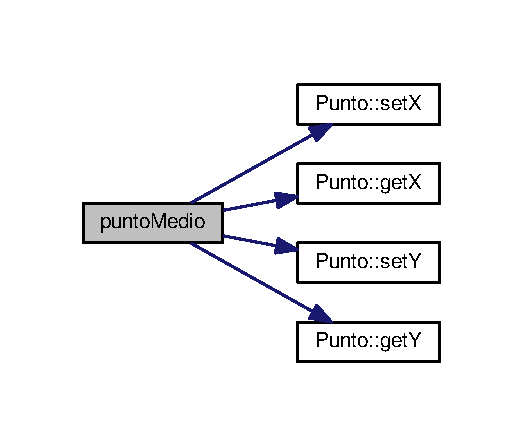
\includegraphics[width=251pt]{circulomedio_8cpp_a119f914f219e98be4c2c93b5138e97da_cgraph}
\end{center}
\end{figure}



%--- End generated contents ---

% Index
\backmatter
\newpage
\phantomsection
\clearemptydoublepage
\addcontentsline{toc}{chapter}{Índice}
\printindex

\end{document}
